\documentclass[11pt,a4paper]{article}

\usepackage[utf8]{inputenc}
\usepackage[T1]{fontenc}
\usepackage[french]{babel}
\usepackage{graphicx}
\usepackage{booktabs}
\usepackage{geometry}
\usepackage{float}
\usepackage{xcolor}
\usepackage{hyperref}
\geometry{margin=2.5cm}
\hypersetup{colorlinks=true, linkcolor=blue, urlcolor=blue}

\title{\textbf{Évaluation de la classification d'émotions de tweets COVID-19}\\
\large Étiquetage automatique par règles \emph{vs} apprentissage automatique :\\
confrontation à une vérité terrain annotée à la main}
\author{Projet EI -- Tweets}
\date{Juin 2026}

\begin{document}

\maketitle

\begin{abstract}
\noindent
Ce rapport complète le travail de prétraitement et de lemmatisation
en se concentrant sur l'\textbf{évaluation} de la classification d'émotions.
Les tweets ont été étiquetés \emph{automatiquement} par un système de règles
(lexique NRC + émojis), puis un modèle d'apprentissage automatique (régression
logistique sur représentation sac-de-mots / TF-IDF) a été entraîné sur ces
étiquettes. Nous évaluons les deux approches contre un jeu de \textbf{297 tweets
annotés manuellement}. Le résultat central est que le modèle reproduit fidèlement
les règles (\textbf{86\,\% d'accord}) mais que \emph{ni les règles ni le modèle ne
correspondent au jugement humain} : leur accuracy ($\approx 23$--$24\,\%$) est
très inférieure à la baseline triviale « toujours \emph{neutral} » ($57\,\%$),
et le $\kappa$ de Cohen est quasi nul. Le facteur limitant est donc la
\emph{qualité de l'étiquetage automatique}, non l'algorithme d'apprentissage.
Une révision des règles (section~\ref{sec:amelioration}) fait ensuite presque
doubler l'accuracy, mais sans gain de $\kappa$ pour les règles : l'amélioration
est surtout mécanique, le ML étant le seul à progresser réellement.
\end{abstract}

\section{Données et représentation}

Le jeu de travail (\texttt{bdd\_etiquetee\_emotions.csv}) contient
\textbf{179\,108} tweets nettoyés et lemmatisés. Chaque ligne comporte :
\begin{itemize}
  \item \texttt{tweet\_lemmatise} : le texte du tweet (nettoyé, lemmatisé) ;
  \item trois variables numériques : \texttt{pct\_majuscules},
        \texttt{exclamations}, \texttt{interrogations} ;
  \item \texttt{emotion} : l'étiquette produite \textbf{automatiquement} par les
        règles (cible d'entraînement) ;
  \item \texttt{Emotion} : l'annotation \textbf{manuelle} (vérité terrain),
        présente sur 297 tweets seulement.
\end{itemize}

\paragraph{Représentation matricielle.}
Le texte est transformé en matrice creuse par \emph{sac de mots} puis pondération
\textbf{TF-IDF} (unigrammes + bigrammes, \texttt{min\_df=2},
\texttt{max\_features=5000}). Les trois variables numériques sont centrées-réduites
(\emph{StandardScaler}) puis concaténées à la matrice TF-IDF. C'est cette matrice
qui alimente le classifieur.

\paragraph{Déséquilibre des classes.}
La figure~\ref{fig:distribution} montre que les deux étiquetages sont dominés par
les classes \emph{neutral} et \emph{anticipation}, les émotions \emph{joy} et
\emph{surprise} étant rares. Ce déséquilibre est traité par l'option
\texttt{class\_weight="balanced"} de la régression logistique.

\begin{figure}[H]
  \centering
  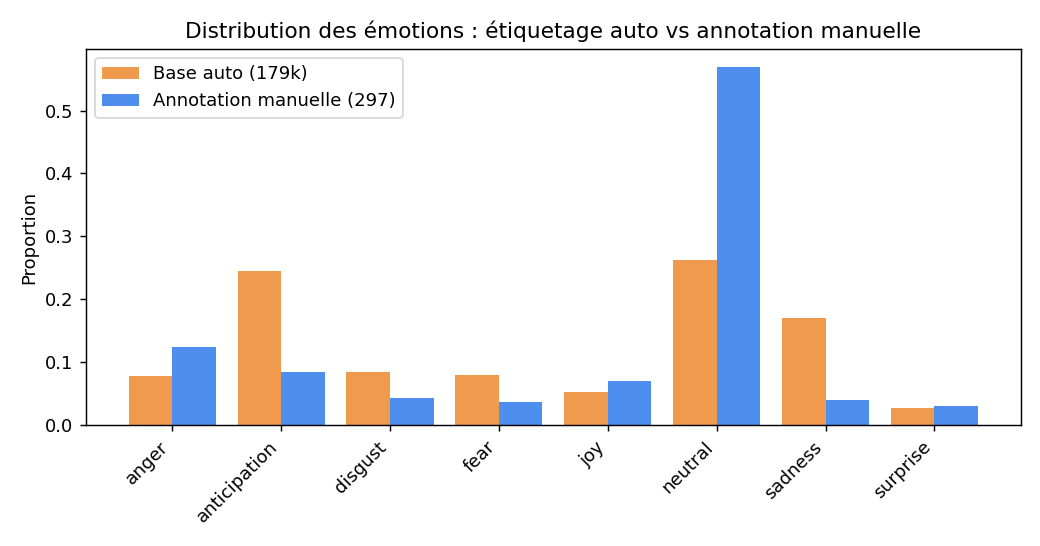
\includegraphics[width=0.85\textwidth]{fig_distribution.png}
  \caption{Distribution des émotions : étiquetage automatique (179k tweets)
  \emph{vs} annotation manuelle (297 tweets).}
  \label{fig:distribution}
\end{figure}

\section{Modèle d'apprentissage}

Le modèle est une \textbf{régression logistique} multinomiale
(\texttt{scikit-learn}), choisie pour sa robustesse en grande dimension et son
\emph{interprétabilité} (on peut lire les mots les plus prédictifs via les
coefficients). Hyperparamètres : \texttt{C=1.0}, \texttt{max\_iter=1000},
\texttt{class\_weight="balanced"}. La chaîne complète (TF-IDF + numériques +
classifieur) est encapsulée dans un \emph{Pipeline} scikit-learn.

\paragraph{Protocole d'évaluation honnête.}
Pour éviter toute fuite de données, le modèle est entraîné sur les
\textbf{178\,811} tweets \emph{non annotés à la main} (en utilisant les étiquettes
automatiques comme cible), puis testé sur les \textbf{297} tweets annotés
manuellement, qui n'ont jamais été vus à l'entraînement. On compare alors, sur ce
même jeu de référence :
\begin{enumerate}
  \item[(A)] les prédictions du \textbf{ML} \emph{vs} l'annotation manuelle ;
  \item[(B)] les étiquettes des \textbf{règles automatiques} \emph{vs}
             l'annotation manuelle.
\end{enumerate}

\section{Résultats}

\begin{table}[H]
  \centering
  \begin{tabular}{lcc}
    \toprule
    \textbf{Prédicteur} & \textbf{Accuracy} & \textbf{$\kappa$ de Cohen} \\
    \midrule
    Baseline « toujours \emph{neutral} » & 0,569 & --- \\
    Règles automatiques \emph{vs} manuel & 0,226 & 0,057 \\
    Machine learning \emph{vs} manuel    & 0,239 & 0,038 \\
    \midrule
    \multicolumn{3}{l}{\emph{Accord ML $\leftrightarrow$ règles auto : 0,859}} \\
    \bottomrule
  \end{tabular}
  \caption{Performances contre la vérité terrain (297 tweets annotés à la main).
  Le $\kappa$ de Cohen mesure l'accord corrigé du hasard ($0$ = hasard,
  $1$ = parfait).}
  \label{tab:resultats}
\end{table}

\begin{figure}[H]
  \centering
  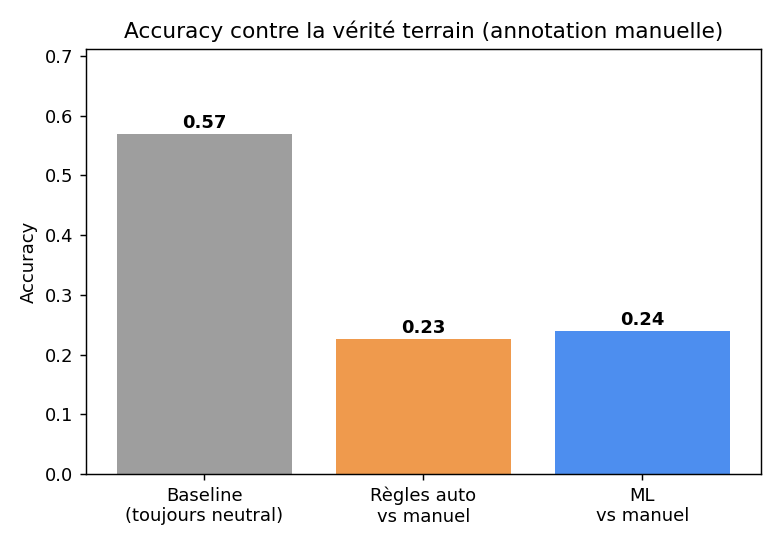
\includegraphics[width=0.7\textwidth]{fig_accuracy.png}
  \caption{Accuracy des deux approches comparée à la baseline triviale.
  Les deux sont \emph{très en dessous} du « toujours \emph{neutral} ».}
  \label{fig:accuracy}
\end{figure}

\begin{figure}[H]
  \centering
  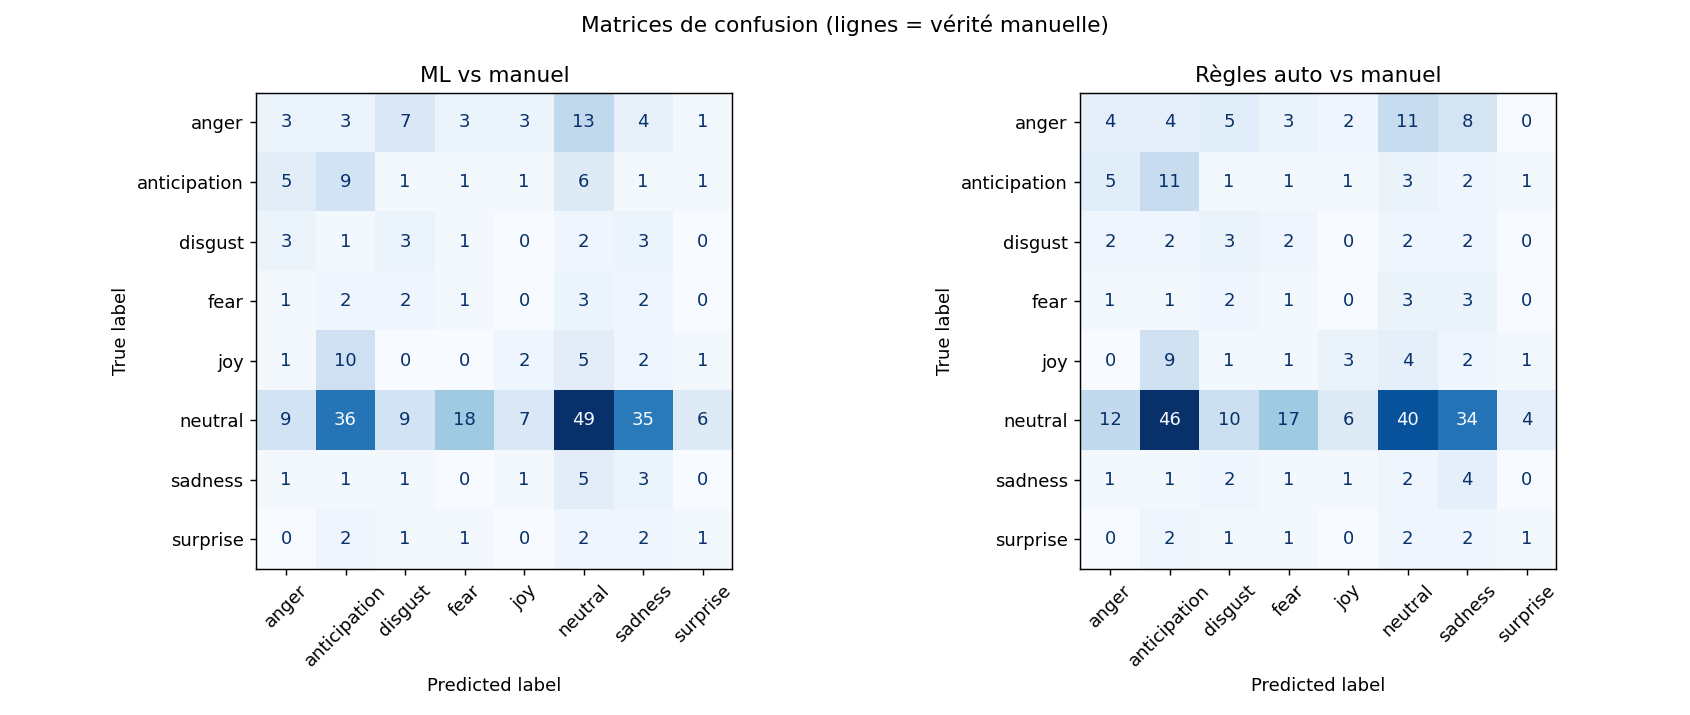
\includegraphics[width=\textwidth]{fig_confusions.png}
  \caption{Matrices de confusion sur les 297 tweets annotés (lignes = vérité
  manuelle, colonnes = prédiction). À gauche le ML, à droite les règles
  automatiques. Les deux dispersent fortement la classe majoritaire
  \emph{neutral}.}
  \label{fig:confusions}
\end{figure}

\section{Interprétation}

\begin{enumerate}
  \item \textbf{Le score élevé obtenu en validation interne était trompeur.}
  Évalué contre ses \emph{propres} étiquettes automatiques, le modèle atteignait
  $\approx 0,86$ d'accuracy. Mais ce chiffre ne mesure que sa \emph{fidélité aux
  règles} : l'accord ML$\leftrightarrow$règles est en effet de $0,859$
  (table~\ref{tab:resultats}), cohérent avec ce $0,86$.

  \item \textbf{Contre la vérité humaine, les deux approches échouent.}
  Avec $\approx 23$--$24\,\%$ d'accuracy, règles et modèle font \emph{moins bien
  qu'un classifieur trivial} prédisant toujours \emph{neutral} ($57\,\%$).
  Le $\kappa$ de Cohen, quasi nul ($\le 0,06$), confirme un accord à peine
  supérieur au hasard.

  \item \textbf{Le ML hérite des défauts de son étiquetage.}
  Comme il apprend à reproduire les règles ($86\,\%$ d'accord), il ne peut pas
  les dépasser : \emph{garbage in, garbage out}. Le problème ne vient donc pas de
  l'algorithme d'apprentissage mais de la \emph{validité de l'étiquetage
  automatique}, qui s'écarte fortement du jugement humain.
\end{enumerate}

\paragraph{Limites.}
Le jeu de référence ne compte que 297 tweets, fortement déséquilibrés
(\emph{surprise}~$=9$, \emph{fear}~$=11$), ce qui rend les métriques par classe
bruitées. Par ailleurs, l'option \texttt{balanced} pénalise l'accuracy brute sur
ce jeu majoritairement neutre, mais ne change pas la conclusion qualitative.

\section{Conclusion et perspectives}

L'étiquetage automatique par règles, bien que reproductible et peu coûteux, ne
reflète pas fidèlement les émotions perçues par un annotateur humain
($\approx 23\,\%$ d'accord, $\kappa \approx 0,06$). Un modèle de régression
logistique entraîné sur ces étiquettes les imite très bien ($86\,\%$) mais hérite
donc de leur faible validité. \textbf{Améliorer le système passe d'abord par
améliorer la qualité des étiquettes} : raffiner les règles, ou — préférablement —
constituer un jeu d'entraînement annoté à la main de taille suffisante et
entraîner directement le modèle dessus. Augmenter la complexité du modèle, à
étiquetage constant, serait sans effet.

\paragraph{Pistes concrètes.}
\begin{itemize}
  \item Étendre l'annotation manuelle (quelques milliers de tweets) et
        entraîner/évaluer le modèle directement dessus (validation croisée).
  \item Comparer plusieurs classifieurs (SVM linéaire, Naïve Bayes) et calibrer
        le seuil de la classe \emph{neutral}.
  \item Auditer les règles d'étiquetage classe par classe à partir des matrices
        de confusion (figure~\ref{fig:confusions}).
\end{itemize}

\section{Amélioration de l'étiquetage : comparaison avant/après}
\label{sec:amelioration}

À la suite de cette analyse, les règles d'étiquetage ont été révisées. La
principale modification est l'introduction d'une règle « \emph{neutral} par
défaut » : une émotion n'est attribuée que si son score dépasse un seuil et
domine nettement les autres ; le vocabulaire COVID factuel (\emph{case},
\emph{death}, \emph{test}, \emph{positive}\ldots) est par ailleurs neutralisé.
La nouvelle base (\texttt{bdd\_etiquetee\_new.csv}) classe ainsi 116\,791 tweets
en \emph{neutral} contre 47\,123 auparavant. Le protocole d'évaluation est
identique (entraînement hors des 297 tweets annotés, test sur ceux-ci).

\begin{table}[H]
  \centering
  \begin{tabular}{lccc}
    \toprule
    \textbf{Indicateur} & \textbf{Ancien} & \textbf{Nouveau} & \textbf{Évol.} \\
    \midrule
    Règles --- accuracy   & 0,226 & \textbf{0,444} & $+0,22$ \\
    Règles --- $\kappa$    & 0,057 & 0,054 & $\approx$ stable \\
    ML --- accuracy        & 0,239 & \textbf{0,354} & $+0,12$ \\
    ML --- $\kappa$        & 0,038 & \textbf{0,094} & $+0,06$ \\
    Accord ML $\leftrightarrow$ règles & 0,859 & 0,660 & --- \\
    \midrule
    \multicolumn{4}{l}{\emph{Baseline « toujours neutral » : 0,569}} \\
    \bottomrule
  \end{tabular}
  \caption{Indicateurs avant/après révision des règles, contre la vérité terrain
  (297 tweets annotés).}
  \label{tab:avant_apres}
\end{table}

\begin{figure}[H]
  \centering
  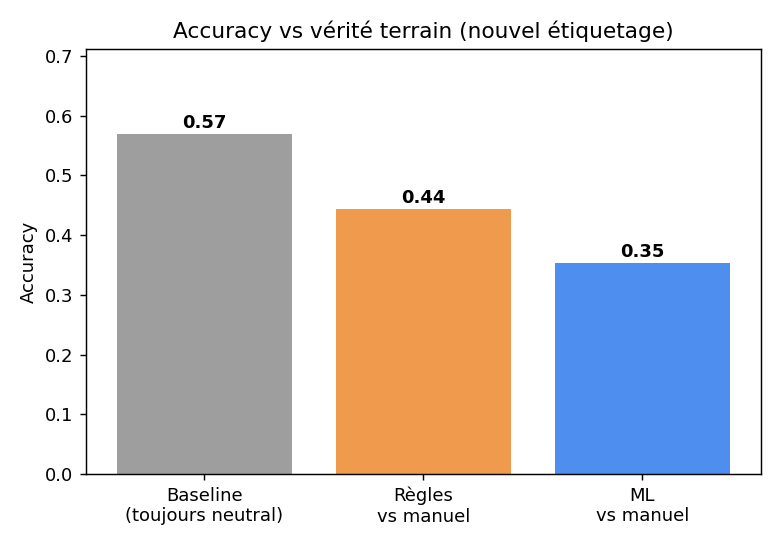
\includegraphics[width=0.7\textwidth]{fig_accuracy_new.png}
  \caption{Accuracy après révision des règles. Le gain est réel mais l'accuracy
  des règles reste sous la baseline triviale.}
  \label{fig:accuracy_new}
\end{figure}

\begin{figure}[H]
  \centering
  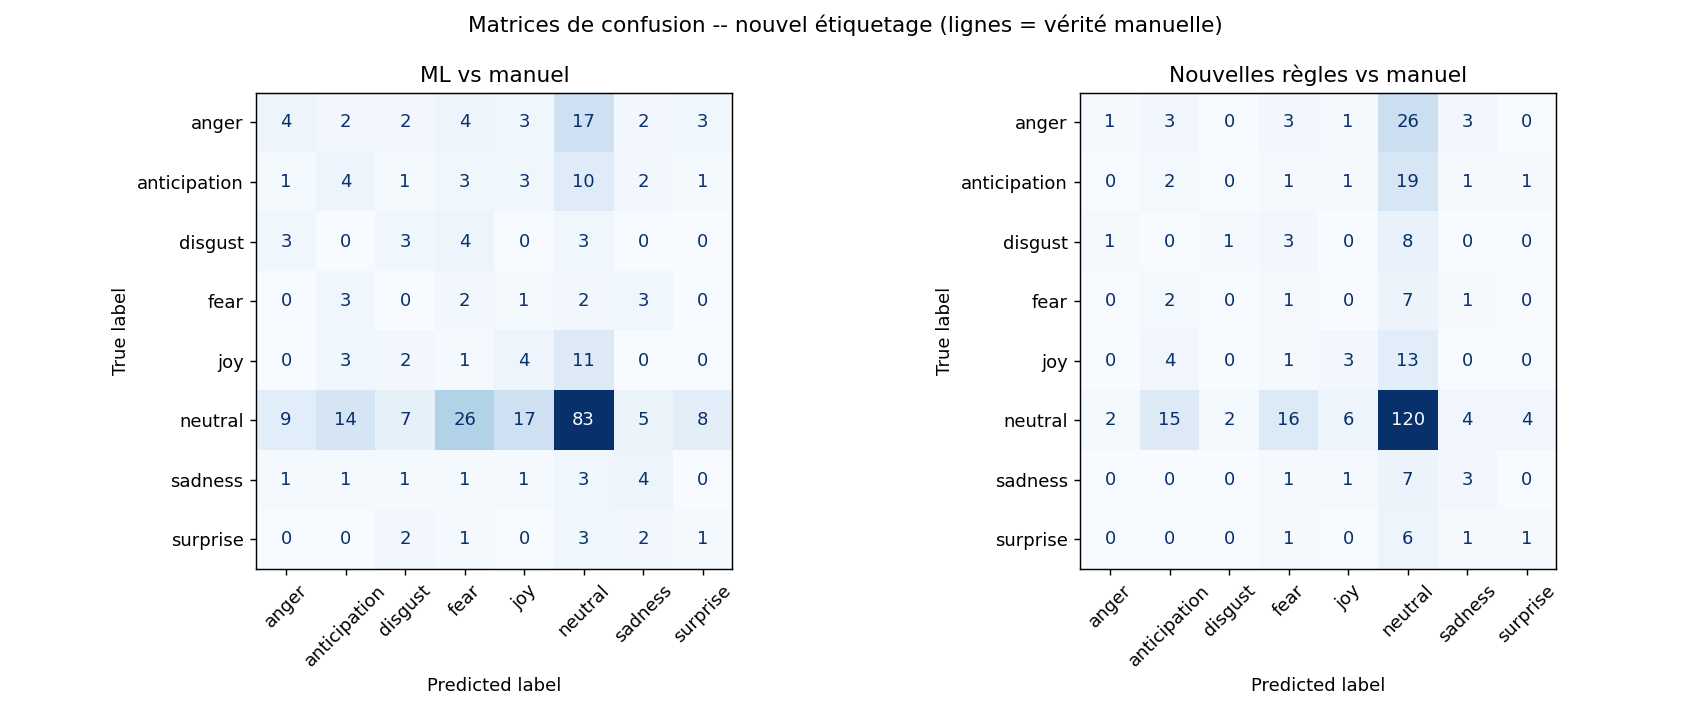
\includegraphics[width=\textwidth]{fig_confusions_new.png}
  \caption{Matrices de confusion après révision (lignes = vérité manuelle). La
  classe \emph{neutral} est désormais bien mieux récupérée.}
  \label{fig:confusions_new}
\end{figure}

\paragraph{Analyse.}
L'accuracy des règles a presque \textbf{doublé} (0,226 $\to$ 0,444) : la règle
« \emph{neutral} par défaut » réduit efficacement le sur-classement des tweets
factuels. \textbf{Cependant}, le $\kappa$ de Cohen reste \emph{plat}
(0,057 $\to$ 0,054). Contrairement à l'accuracy, le $\kappa$ corrige du hasard :
ce gain d'accuracy est donc en grande partie \emph{mécanique}, dû au fait que les
règles prédisent plus souvent la classe majoritaire \emph{neutral} (57\,\% du jeu
de test). En accuracy pure, les règles (0,444) restent d'ailleurs
\emph{en dessous} de la baseline « toujours \emph{neutral} » (0,569).

En revanche, le modèle de ML progresse réellement sur le $\kappa$
(0,038 $\to$ 0,094, soit $\times 2,5$) : c'est le seul indicateur traduisant une
amélioration \emph{authentique} de la discrimination entre émotions, même si elle
demeure modeste. La baisse de l'accord ML$\leftrightarrow$règles (0,859 $\to$
0,660) confirme que le ML ne se contente plus de recopier les règles.

\paragraph{Conséquence.} Les nouvelles règles réduisent le bruit (moins de
fausses émotions), ce qui bénéficie au ML, mais le font surtout en
« jouant la sécurité » sur \emph{neutral}. Le prochain levier est de mieux
\emph{discriminer les émotions entre elles} (règles ciblées par émotion :
\emph{anger}, \emph{fear}, \emph{joy}\ldots), seul moyen de faire progresser le
$\kappa$.

\appendix
\section{Reproductibilité}
\begin{itemize}
  \item \texttt{machine\_learning.py} : modèle de référence (jeu annoté à la main).
  \item \texttt{machine\_learning\_auto.py} : modèle entraîné sur l'étiquetage
        automatique, test sur les 50\,000 derniers tweets.
  \item \texttt{evaluation\_ml.py} : comparaison ML \emph{vs} règles contre la
        vérité manuelle (rapports détaillés par classe).
  \item \texttt{rapport\_figures.py} : génération des figures et métriques de la
        section principale.
  \item \texttt{evaluation\_new.py} : reprise des mêmes indicateurs sur le nouvel
        étiquetage (\texttt{bdd\_etiquetee\_new.csv}), figures \texttt{*\_new.png}
        de la section~\ref{sec:amelioration}.
\end{itemize}
Environnement : Python 3.10, scikit-learn 1.7, pandas 2.3, matplotlib 3.10.

\end{document}
